\documentclass{standalone}
\usepackage{tikz}
\usetikzlibrary{patterns, positioning}
\usepackage[sfdefault]{ClearSans} %% option 'sfdefault' activates Clear Sans as the default text font
\usepackage[T1]{fontenc}

\begin{document}
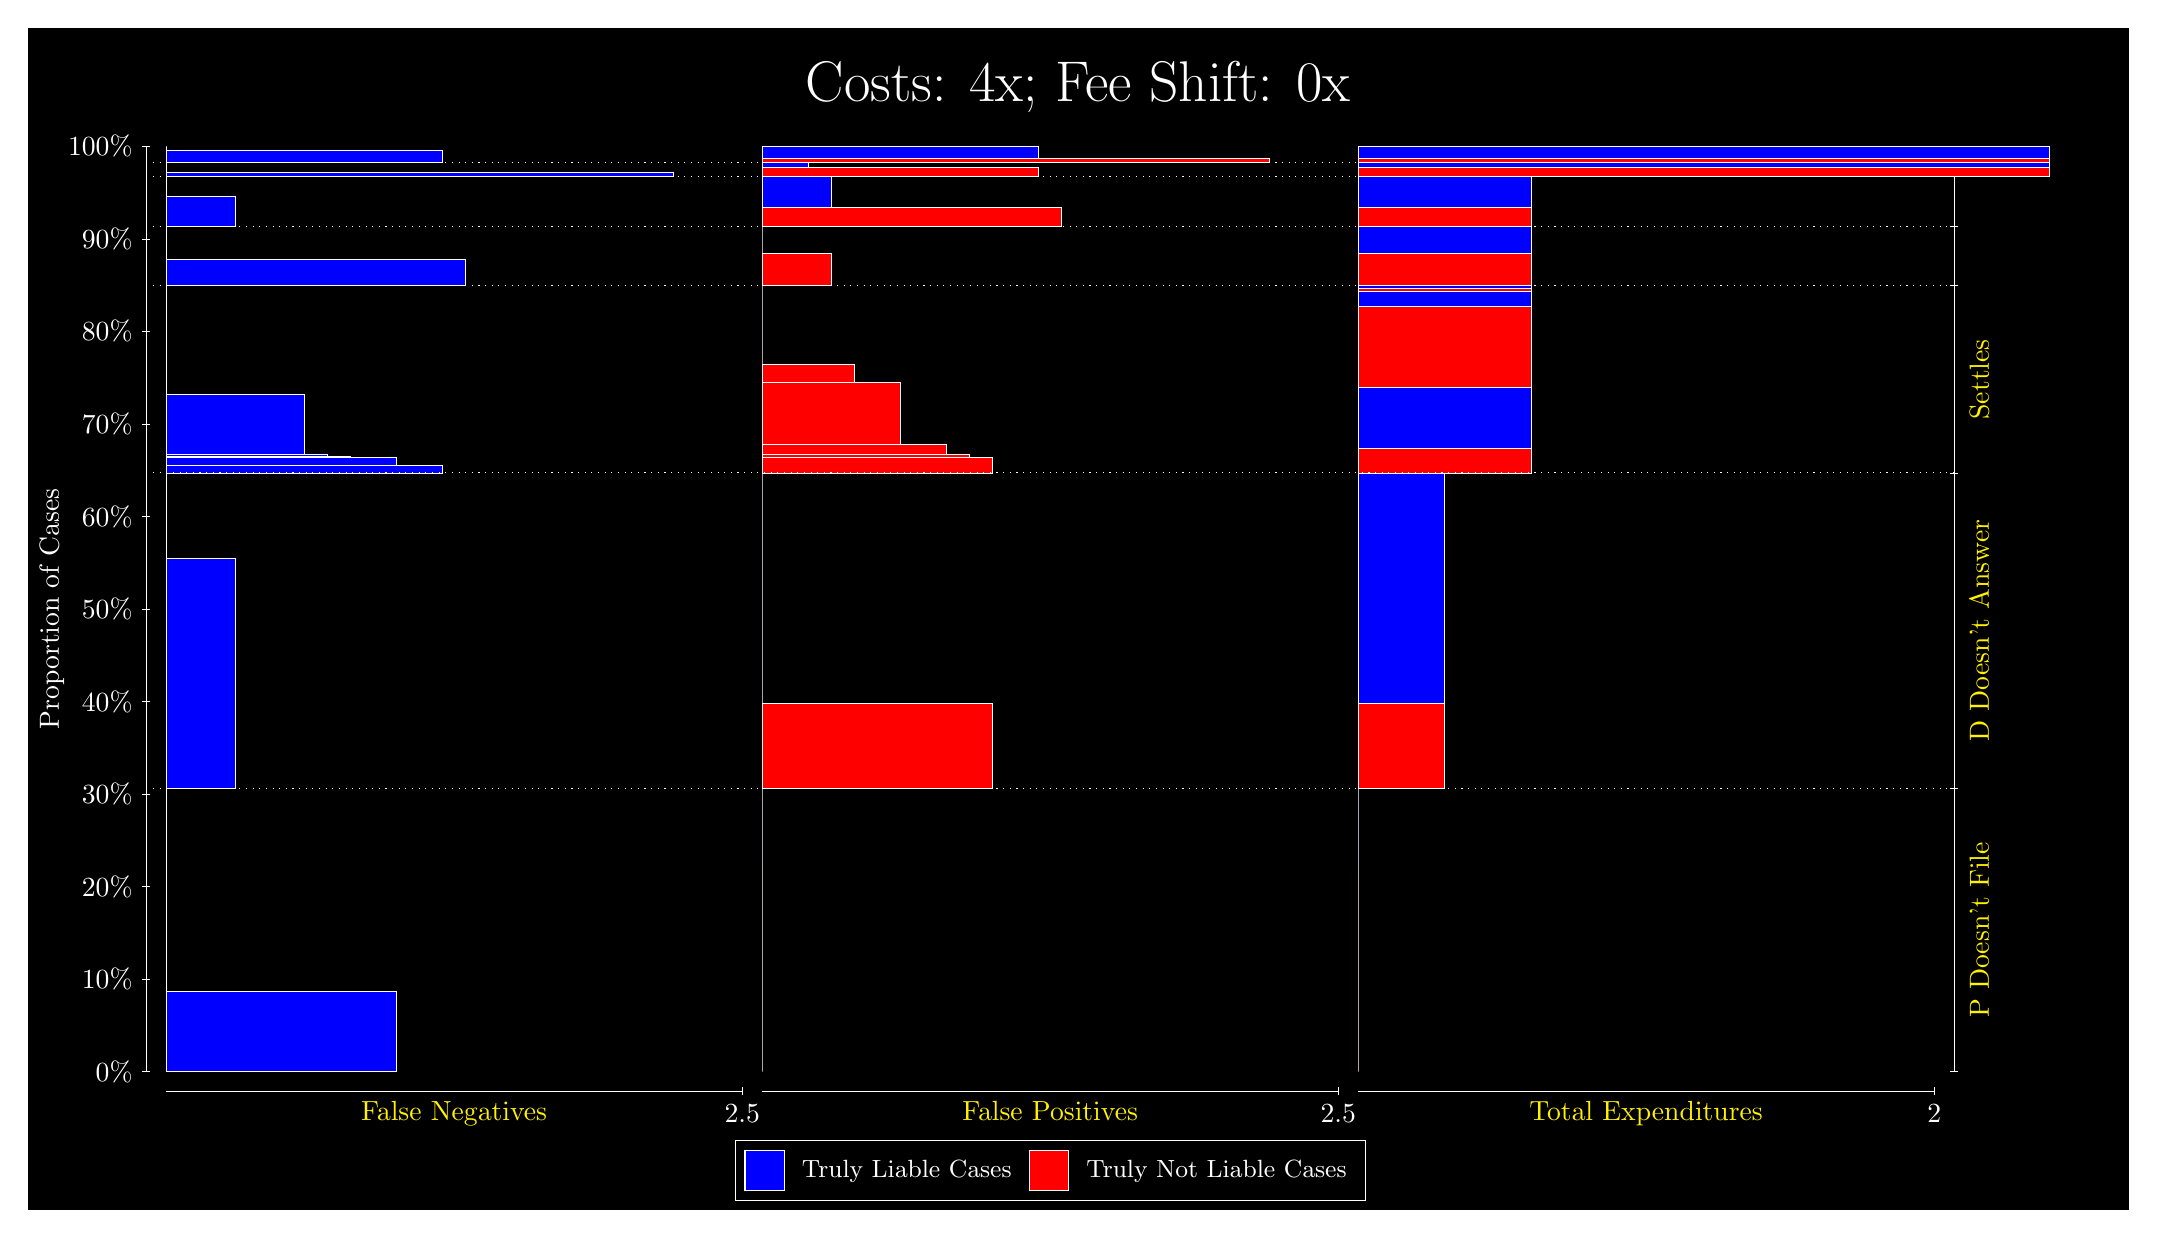
\begin{tikzpicture}
\draw[fill=black] (0,0) rectangle (26.667,15);
\draw[text=white] (0,13.5) rectangle (26.667,15) node[midway] {\huge Costs: 4x; Fee Shift: 0x};
\draw[white, very thin] (1.5,1.75) -- (1.5,13.5);
\node[rotate=90, text=white, anchor=center] at (0.3, 7.625) {Proportion of Cases};
\draw[white, very thin] (1.45,1.75) -- (1.55,1.75);
\node[text=white, anchor=east] at (1.45, 1.75) {0\%};
\draw[white, very thin] (1.45,2.925) -- (1.55,2.925);
\node[text=white, anchor=east] at (1.45, 2.925) {10\%};
\draw[white, very thin] (1.45,4.1) -- (1.55,4.1);
\node[text=white, anchor=east] at (1.45, 4.1) {20\%};
\draw[white, very thin] (1.45,5.275) -- (1.55,5.275);
\node[text=white, anchor=east] at (1.45, 5.275) {30\%};
\draw[white, very thin] (1.45,6.45) -- (1.55,6.45);
\node[text=white, anchor=east] at (1.45, 6.45) {40\%};
\draw[white, very thin] (1.45,7.625) -- (1.55,7.625);
\node[text=white, anchor=east] at (1.45, 7.625) {50\%};
\draw[white, very thin] (1.45,8.8) -- (1.55,8.8);
\node[text=white, anchor=east] at (1.45, 8.8) {60\%};
\draw[white, very thin] (1.45,9.975) -- (1.55,9.975);
\node[text=white, anchor=east] at (1.45, 9.975) {70\%};
\draw[white, very thin] (1.45,11.15) -- (1.55,11.15);
\node[text=white, anchor=east] at (1.45, 11.15) {80\%};
\draw[white, very thin] (1.45,12.325) -- (1.55,12.325);
\node[text=white, anchor=east] at (1.45, 12.325) {90\%};
\draw[white, very thin] (1.45,13.5) -- (1.55,13.5);
\node[text=white, anchor=east] at (1.45, 13.5) {100\%};

\draw[white, very thin] (24.457,1.75) -- (24.457,13.5);
\draw[white, very thin] (24.407,1.75) -- (24.507,1.75);
\node[anchor=west] at (24.407, 1.75) {};
\draw[white, very thin] (24.407,5.3438) -- (24.507,5.3438);
\node[anchor=west] at (24.407, 5.3438) {};
\draw[white, very thin] (24.407,9.3536) -- (24.507,9.3536);
\node[anchor=west] at (24.407, 9.3536) {};
\draw[white, very thin] (24.407,11.729) -- (24.507,11.729);
\node[anchor=west] at (24.407, 11.729) {};
\draw[white, very thin] (24.407,12.48) -- (24.507,12.48);
\node[anchor=west] at (24.407, 12.48) {};
\draw[white, very thin] (24.407,13.119) -- (24.507,13.119);
\node[anchor=west] at (24.407, 13.119) {};
\draw[white, very thin] (24.407,13.293) -- (24.507,13.293);
\node[anchor=west] at (24.407, 13.293) {};
\draw[white, very thin] (24.407,13.5) -- (24.507,13.5);
\node[anchor=west] at (24.407, 13.5) {};

\draw[white, very thin, fill=blue] (1.75,1.75) rectangle (4.6775,2.7737);
\draw[white, very thin, fill=red] (1.75,2.7737) rectangle (1.75,5.3438);
\draw[white, very thin, fill=blue] (1.75,5.3438) rectangle (2.6283,8.2668);
\draw[white, very thin, fill=red] (1.75,8.2668) rectangle (1.75,9.3536);
\draw[white, very thin, fill=blue] (1.75,9.3536) rectangle (5.2631,9.4467);
\draw[white, very thin, fill=blue] (1.75,9.4467) rectangle (4.6775,9.5457);
\draw[white, very thin, fill=blue] (1.75,9.5457) rectangle (4.092,9.568);
\draw[white, very thin, fill=blue] (1.75,9.568) rectangle (3.7993,9.5938);
\draw[white, very thin, fill=blue] (1.75,9.5938) rectangle (3.5065,10.353);
\draw[white, very thin, fill=red] (1.75,10.353) rectangle (1.75,11.729);
\draw[white, very thin, fill=blue] (1.75,11.729) rectangle (5.5558,12.063);
\draw[white, very thin, fill=red] (1.75,12.063) rectangle (1.75,12.48);
\draw[white, very thin, fill=blue] (1.75,12.48) rectangle (2.6283,12.868);
\draw[white, very thin, fill=red] (1.75,12.868) rectangle (1.75,13.119);
\draw[white, very thin, fill=blue] (1.75,13.119) rectangle (8.1906,13.175);
\draw[white, very thin, fill=red] (1.75,13.175) rectangle (1.75,13.293);
\draw[white, very thin, fill=blue] (1.75,13.293) rectangle (5.2631,13.444);
\draw[white, very thin, fill=red] (1.75,13.444) rectangle (1.75,13.5);
\draw[white, very thin, fill=red] (9.3189,1.75) rectangle (9.3189,4.3201);
\draw[white, very thin, fill=blue] (9.3189,4.3201) rectangle (9.3189,5.3438);
\draw[white, very thin, fill=red] (9.3189,5.3438) rectangle (12.246,6.4305);
\draw[white, very thin, fill=blue] (9.3189,6.4305) rectangle (9.3189,9.3536);
\draw[white, very thin, fill=red] (9.3189,9.3536) rectangle (12.246,9.5447);
\draw[white, very thin, fill=red] (9.3189,9.5447) rectangle (11.954,9.5912);
\draw[white, very thin, fill=red] (9.3189,9.5912) rectangle (11.661,9.711);
\draw[white, very thin, fill=red] (9.3189,9.711) rectangle (11.075,10.506);
\draw[white, very thin, fill=red] (9.3189,10.506) rectangle (10.49,10.73);
\draw[white, very thin, fill=blue] (9.3189,10.73) rectangle (9.3189,11.729);
\draw[white, very thin, fill=red] (9.3189,11.729) rectangle (10.197,12.145);
\draw[white, very thin, fill=blue] (9.3189,12.145) rectangle (9.3189,12.48);
\draw[white, very thin, fill=red] (9.3189,12.48) rectangle (13.125,12.731);
\draw[white, very thin, fill=blue] (9.3189,12.731) rectangle (10.197,13.119);
\draw[white, very thin, fill=red] (9.3189,13.119) rectangle (12.832,13.237);
\draw[white, very thin, fill=blue] (9.3189,13.237) rectangle (9.9044,13.293);
\draw[white, very thin, fill=red] (9.3189,13.293) rectangle (15.759,13.349);
\draw[white, very thin, fill=blue] (9.3189,13.349) rectangle (12.832,13.5);
\draw[white, very thin, fill=red] (16.888,1.75) rectangle (16.888,4.3201);
\draw[white, very thin, fill=blue] (16.888,4.3201) rectangle (16.888,5.3438);
\draw[white, very thin, fill=red] (16.888,5.3438) rectangle (17.986,6.4305);
\draw[white, very thin, fill=blue] (16.888,6.4305) rectangle (17.986,9.3536);
\draw[white, very thin, fill=red] (16.888,9.3536) rectangle (19.083,9.6645);
\draw[white, very thin, fill=blue] (16.888,9.6645) rectangle (19.083,10.446);
\draw[white, very thin, fill=red] (16.888,10.446) rectangle (19.083,11.464);
\draw[white, very thin, fill=blue] (16.888,11.464) rectangle (19.083,11.656);
\draw[white, very thin, fill=red] (16.888,11.656) rectangle (19.083,11.703);
\draw[white, very thin, fill=blue] (16.888,11.703) rectangle (19.083,11.729);
\draw[white, very thin, fill=red] (16.888,11.729) rectangle (19.083,12.145);
\draw[white, very thin, fill=blue] (16.888,12.145) rectangle (19.083,12.48);
\draw[white, very thin, fill=red] (16.888,12.48) rectangle (19.083,12.731);
\draw[white, very thin, fill=blue] (16.888,12.731) rectangle (19.083,13.119);
\draw[white, very thin, fill=red] (16.888,13.119) rectangle (25.67,13.237);
\draw[white, very thin, fill=blue] (16.888,13.237) rectangle (25.67,13.293);
\draw[white, very thin, fill=red] (16.888,13.293) rectangle (25.67,13.349);
\draw[white, very thin, fill=blue] (16.888,13.349) rectangle (25.67,13.5);
\draw[white, dotted] (1.5,5.3438) -- (24.457,5.3438);
\draw[white, dotted] (1.5,9.3536) -- (24.457,9.3536);
\draw[white, dotted] (1.5,11.729) -- (24.457,11.729);
\draw[white, dotted] (1.5,12.48) -- (24.457,12.48);
\draw[white, dotted] (1.5,13.119) -- (24.457,13.119);
\draw[white, dotted] (1.5,13.293) -- (24.457,13.293);
\draw[white, very thin] (1.75,1.5) -- (9.0689,1.5);
\node[text=yellow, anchor=north] at (5.4094, 1.5) {False Negatives};
\draw[white, very thin] (9.0689,1.45) -- (9.0689,1.55);
\node[text=white, anchor=north] at (9.0689, 1.45) {2.5};

\draw[white, very thin] (9.3189,1.5) -- (16.638,1.5);
\node[text=yellow, anchor=north] at (12.978, 1.5) {False Positives};
\draw[white, very thin] (16.638,1.45) -- (16.638,1.55);
\node[text=white, anchor=north] at (16.638, 1.45) {2.5};

\draw[white, very thin] (16.888,1.5) -- (24.207,1.5);
\node[text=yellow, anchor=north] at (20.547, 1.5) {Total Expenditures};
\draw[white, very thin] (24.207,1.45) -- (24.207,1.55);
\node[text=white, anchor=north] at (24.207, 1.45) {2};

\node[text=yellow, centered, rotate=90] at (24.777, 3.5469) {P Doesn't File};
\node[text=yellow, centered, rotate=90] at (24.777, 7.3487) {D Doesn't Answer};
\node[text=yellow, centered, rotate=90] at (24.777, 10.541) {Settles};





\draw (12.978300999999998,1.5) node[draw=none] (baseCoordinate) {};
\begin{scope}[align=center]
        \matrix[scale=0.5, draw=white, below=0.5cm of baseCoordinate, nodes={draw}, column sep=0.1cm]{
            \node[rectangle, draw, minimum width=0.5cm, minimum height=0.5cm, fill=blue] {}; &
            \node[draw=none, font=\small, text=white] (B) {Truly Liable Cases}; &
            \node[rectangle, draw, minimum width=0.5cm, minimum height=0.5cm, fill=red] {}; &
            \node[draw=none, font=\small, text=white] (B) {Truly Not Liable Cases}; \\
            };
\end{scope}

\end{tikzpicture}
\end{document}